\documentclass[varwidth=7in]{standalone}
\usepackage{tikz,mwe}
\usetikzlibrary{calc,decorations.pathmorphing}
\begin{document}
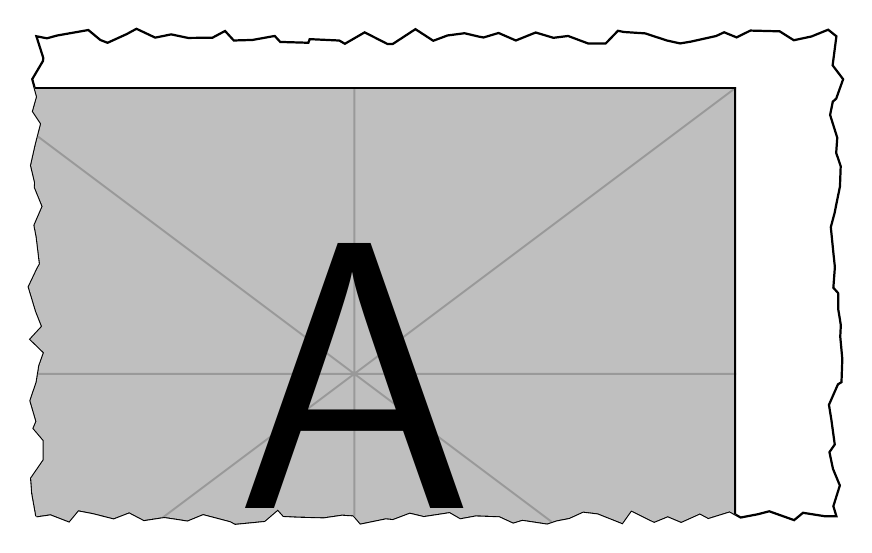
\begin{tikzpicture}[scale=0.8]
\pgfmathsetmacro\myScale{0.8} % Set this to the same as the preceding value
\pgfmathsetmacro\myW{5}
\pgfmathsetmacro\myH{3}
\pgfmathsetmacro\myX{0.4}
\pgfmathsetmacro\myY{0.9}
\clip[preaction={draw, line width=.8pt}] (\myX in, \myY in) decorate[decoration={random steps,segment length=2mm,amplitude=.1cm}] {(\myX in, \myY in) --++ (\myW in, 0) --++ (0, \myH in) --++ (-\myW in, 0) --++ (0, -\myH in)};
\node[inner sep=0, outer sep=0, anchor=south west] (image) at (0, 0) {\includegraphics[width=\myScale\textwidth]{example-image-a}};
\end{tikzpicture}
\end{document}